\begin{appendices}
\chapter{}
\label{appendix:text}


\chapter{Trial Summary Plots by Subject}
\label{appendix:SubjectSummary}
\newcommand\plotHeight{0.8}
% Subject A
\begin{figure}[hbt!]
    \centering
    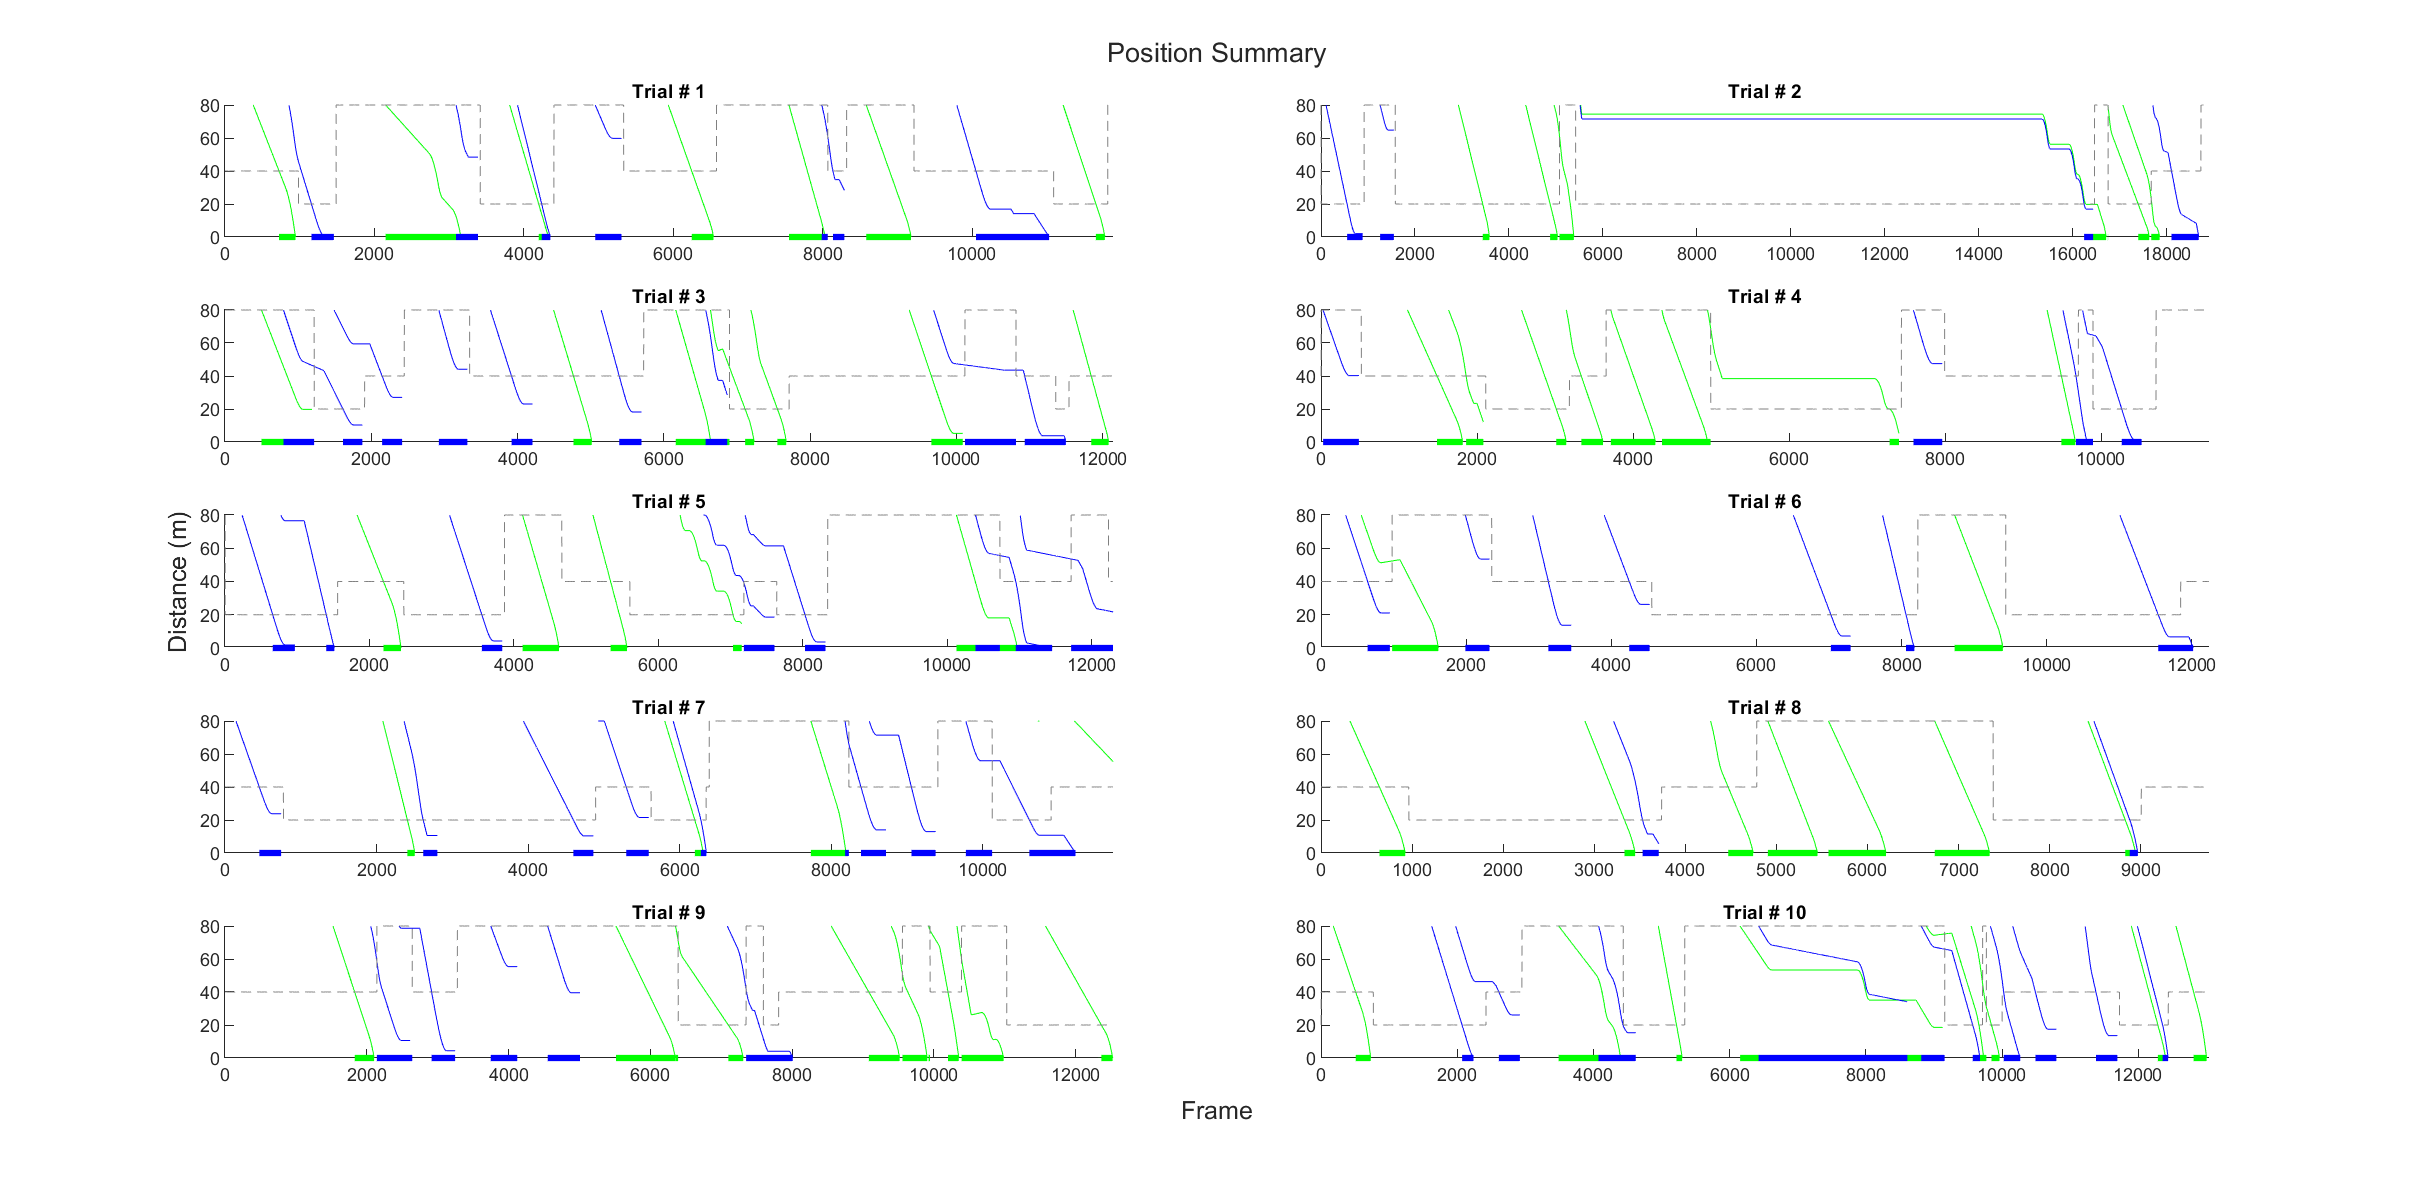
\includegraphics[width=\linewidth, height=\plotHeight\linewidth]{figures/subject_a_summary.eps}
    \caption{Summary Plot of Subject A's Trials}
    \label{fig:SumA}
\end{figure}

% Subject B
\begin{figure}[hbt!]
    \centering
    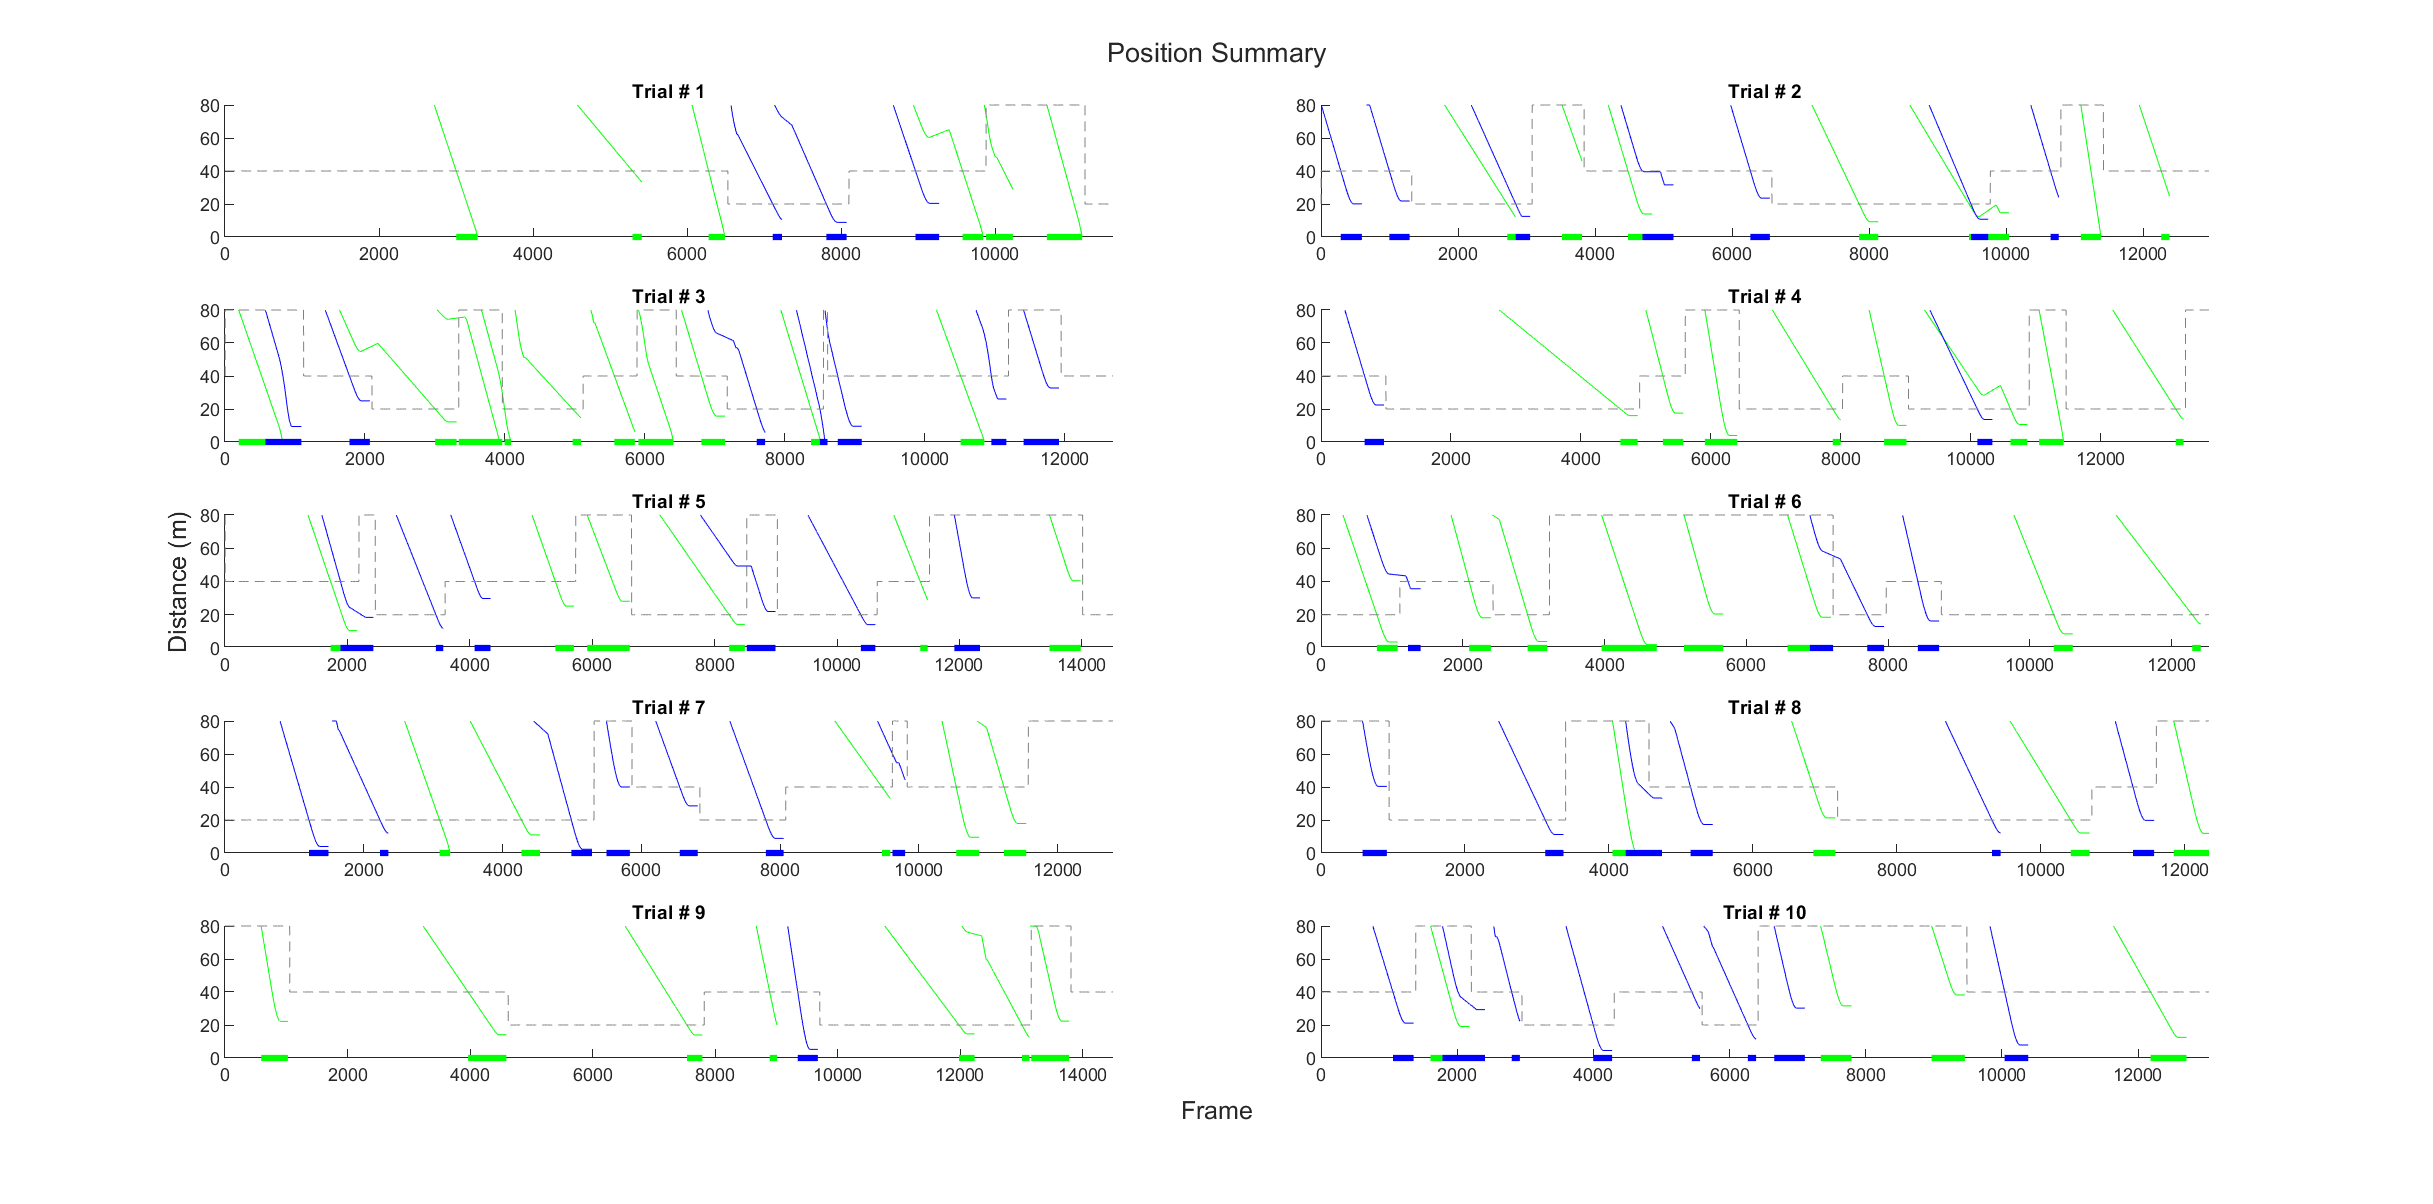
\includegraphics[width=\linewidth, height=\plotHeight\linewidth]{figures/subject_b_summary.eps}
    \caption{Summary Plot of Subject B's Trials}
    \label{fig:SumB}
\end{figure}

% Subject C
\begin{figure}[hbt!]
    \centering
    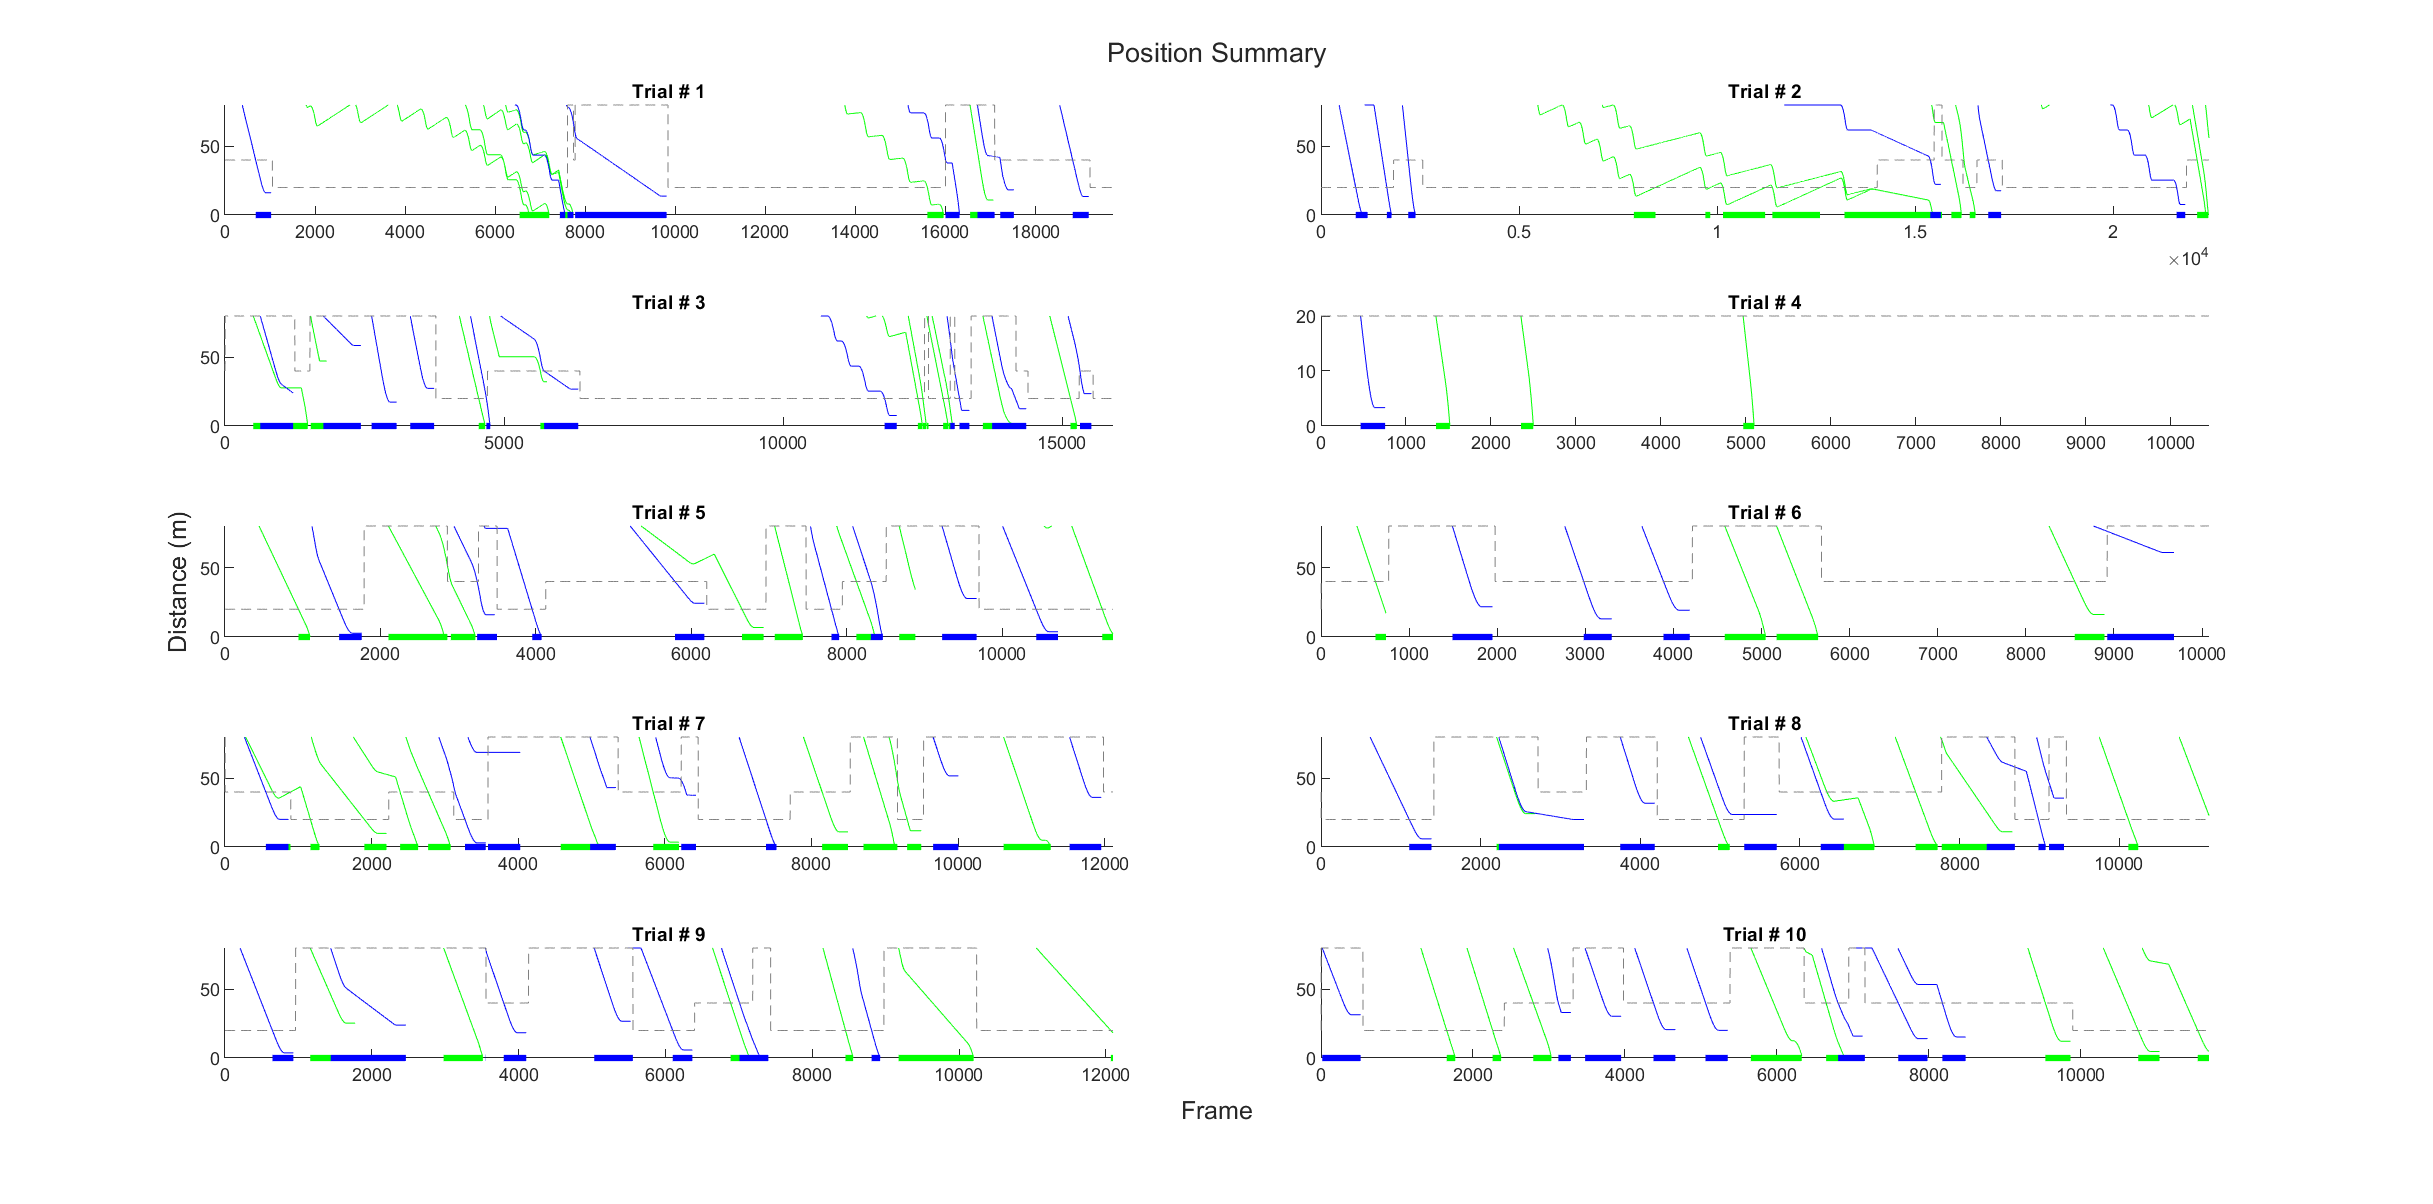
\includegraphics[width=\linewidth, height=\plotHeight\linewidth]{figures/subject_c_summary.eps}
    \caption{Summary Plot of Subject C's Trials}
    \label{fig:SumC}
\end{figure}

% Subject D
\begin{figure}[hbt!]
    \centering
    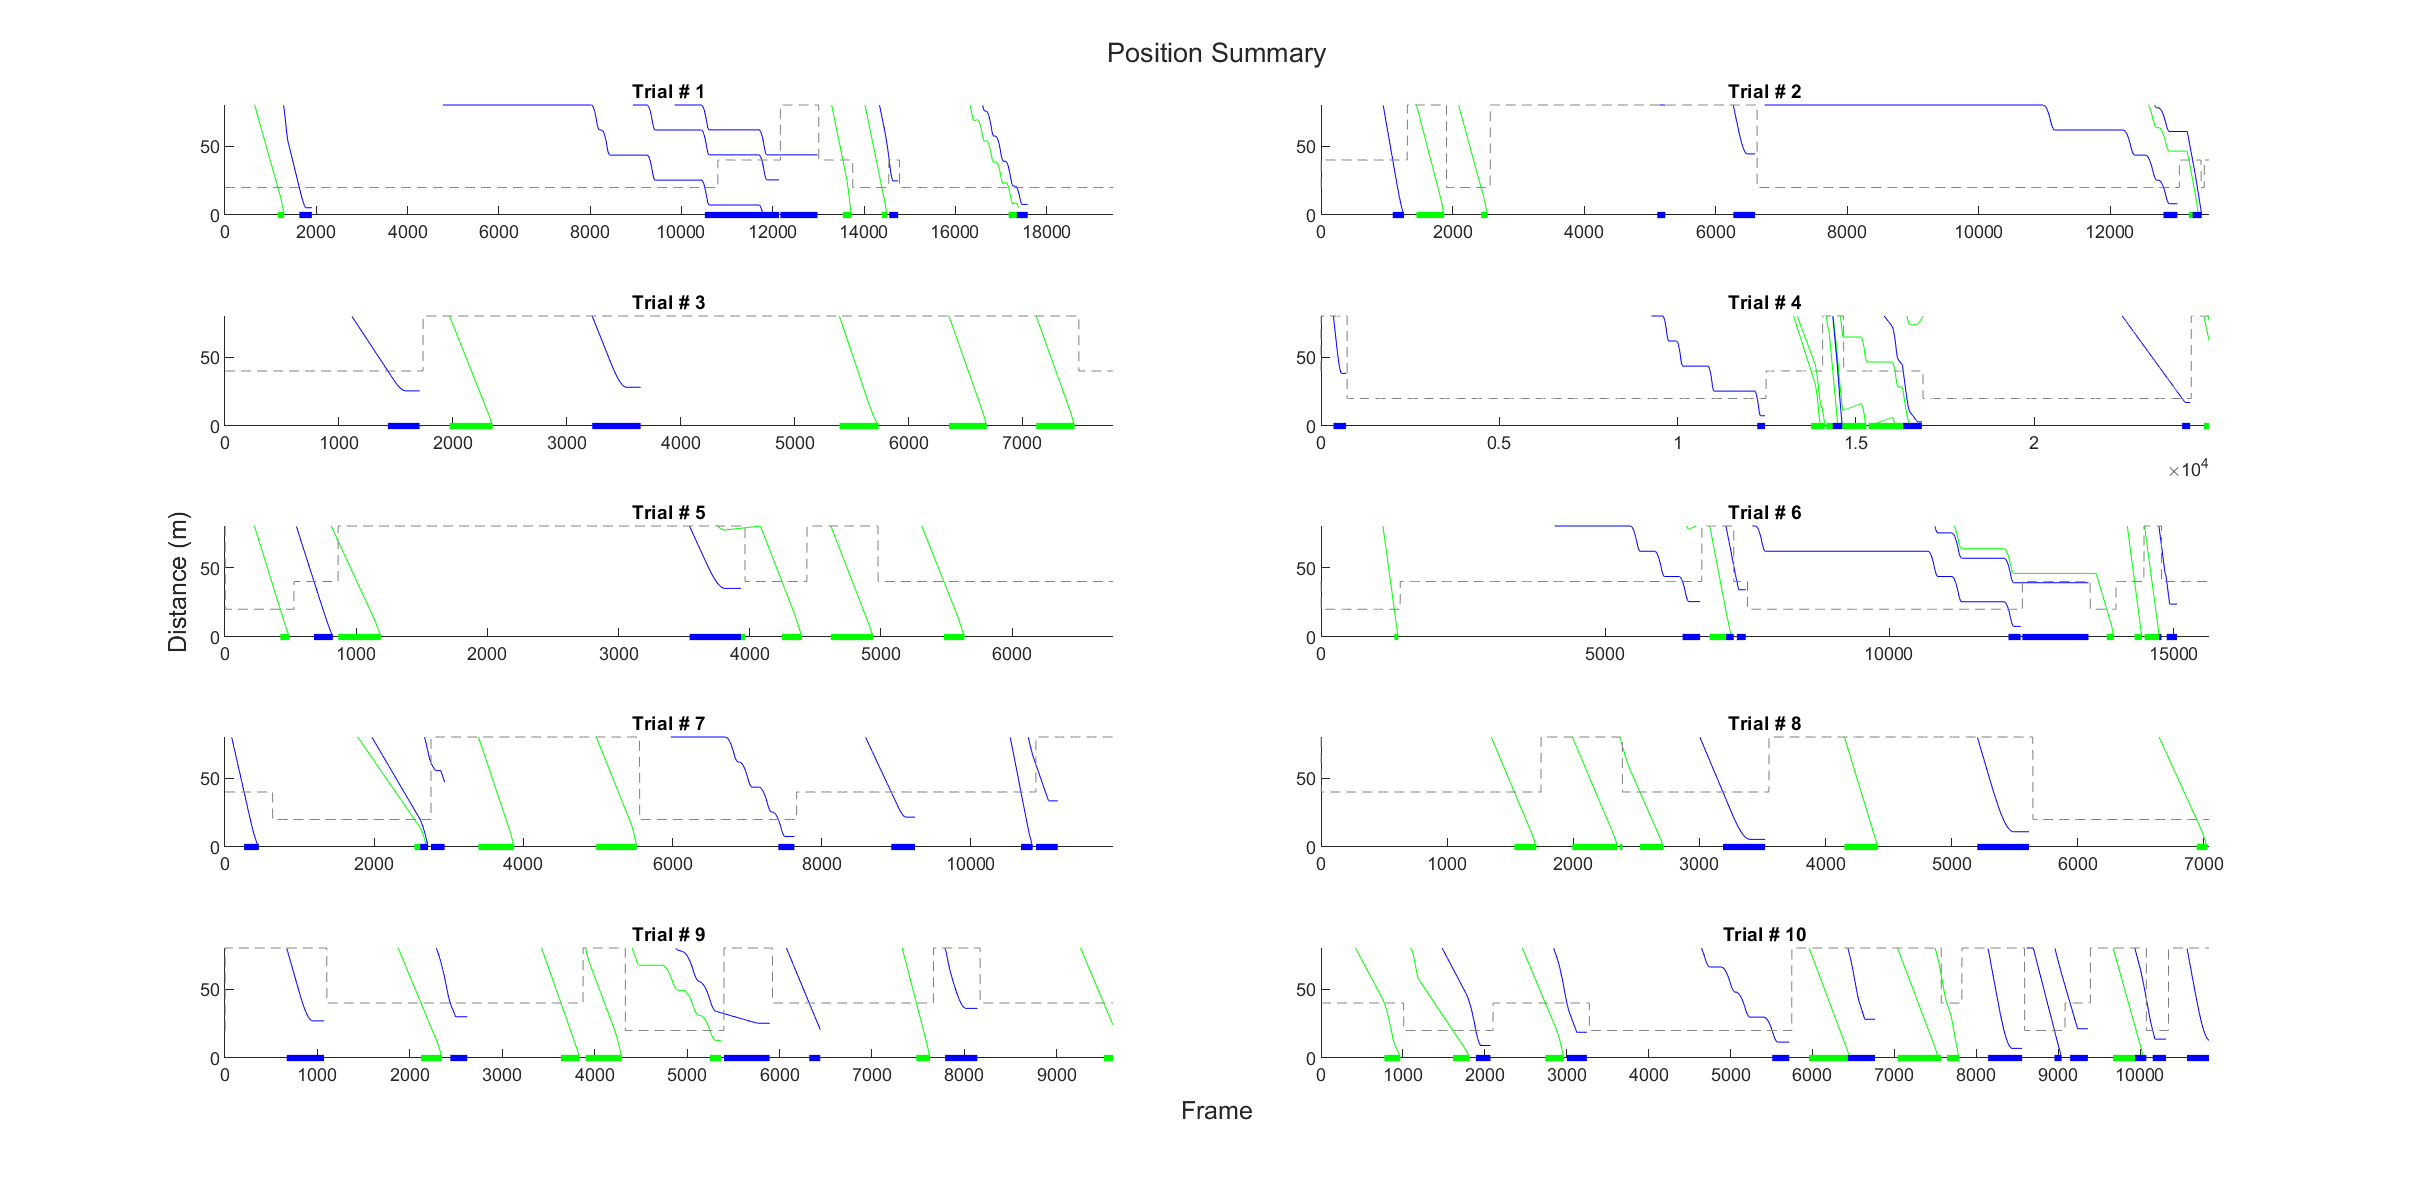
\includegraphics[width=\linewidth, height=\plotHeight\linewidth]{figures/subject_d_summary.eps}
    \caption{Summary Plot of Subject D's Trials}
    \label{fig:SumD}
\end{figure}

% Subject E
\begin{figure}[hbt!]
    \centering
    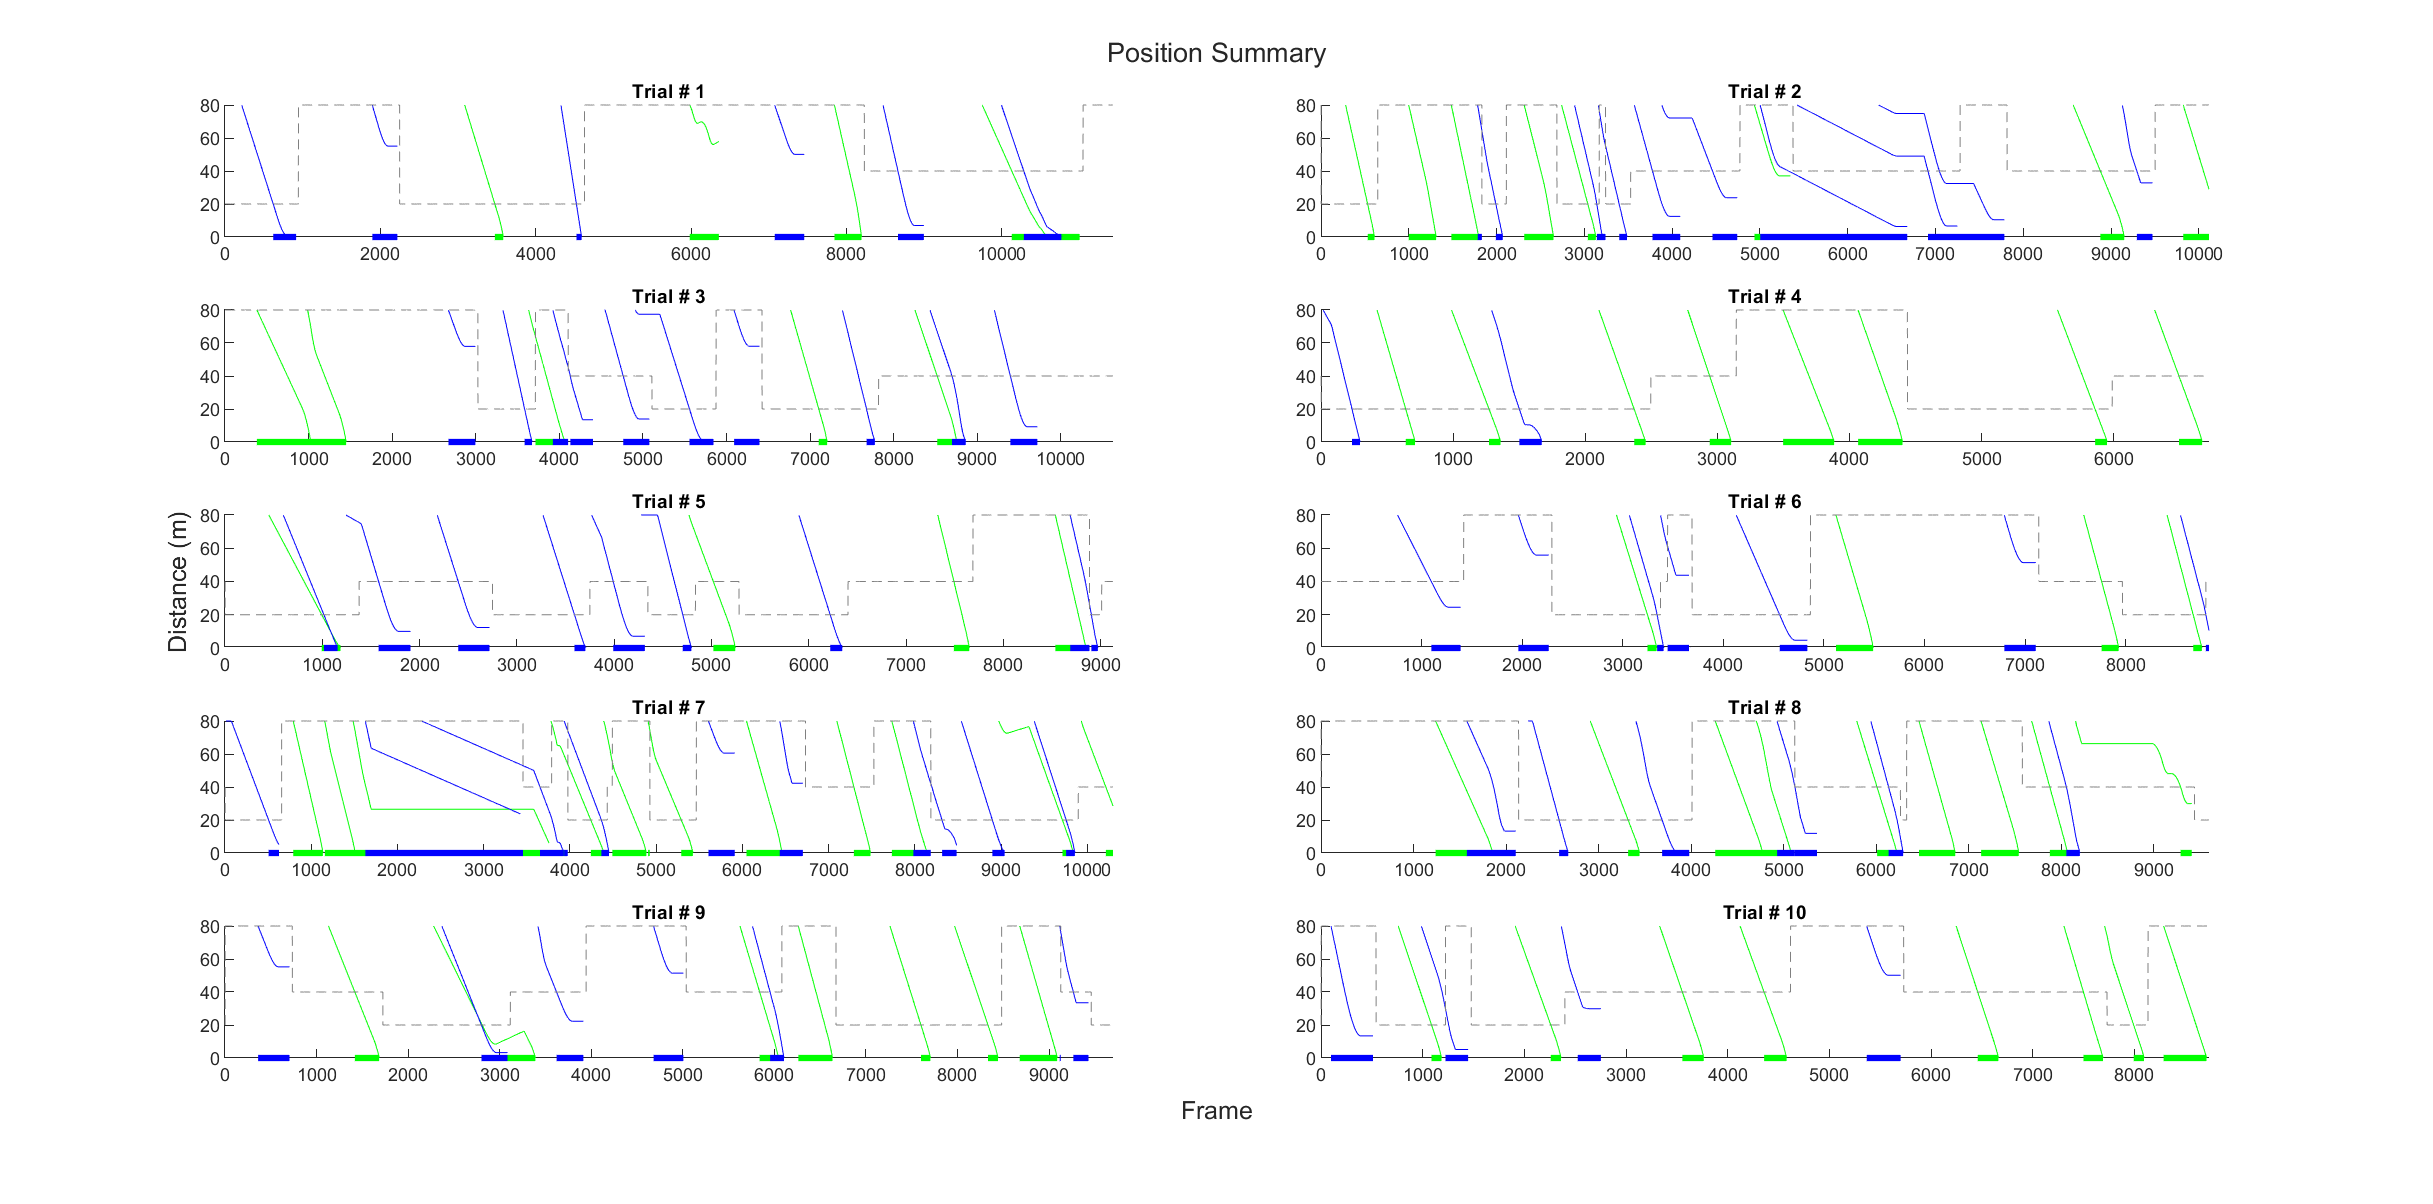
\includegraphics[width=\linewidth, height=\plotHeight\linewidth]{figures/subject_e_summary.eps}
    \caption{Summary Plot of Subject E's Trials}
    \label{fig:SumE}
\end{figure}

% Subject F
\begin{figure}[hbt!]
    \centering
    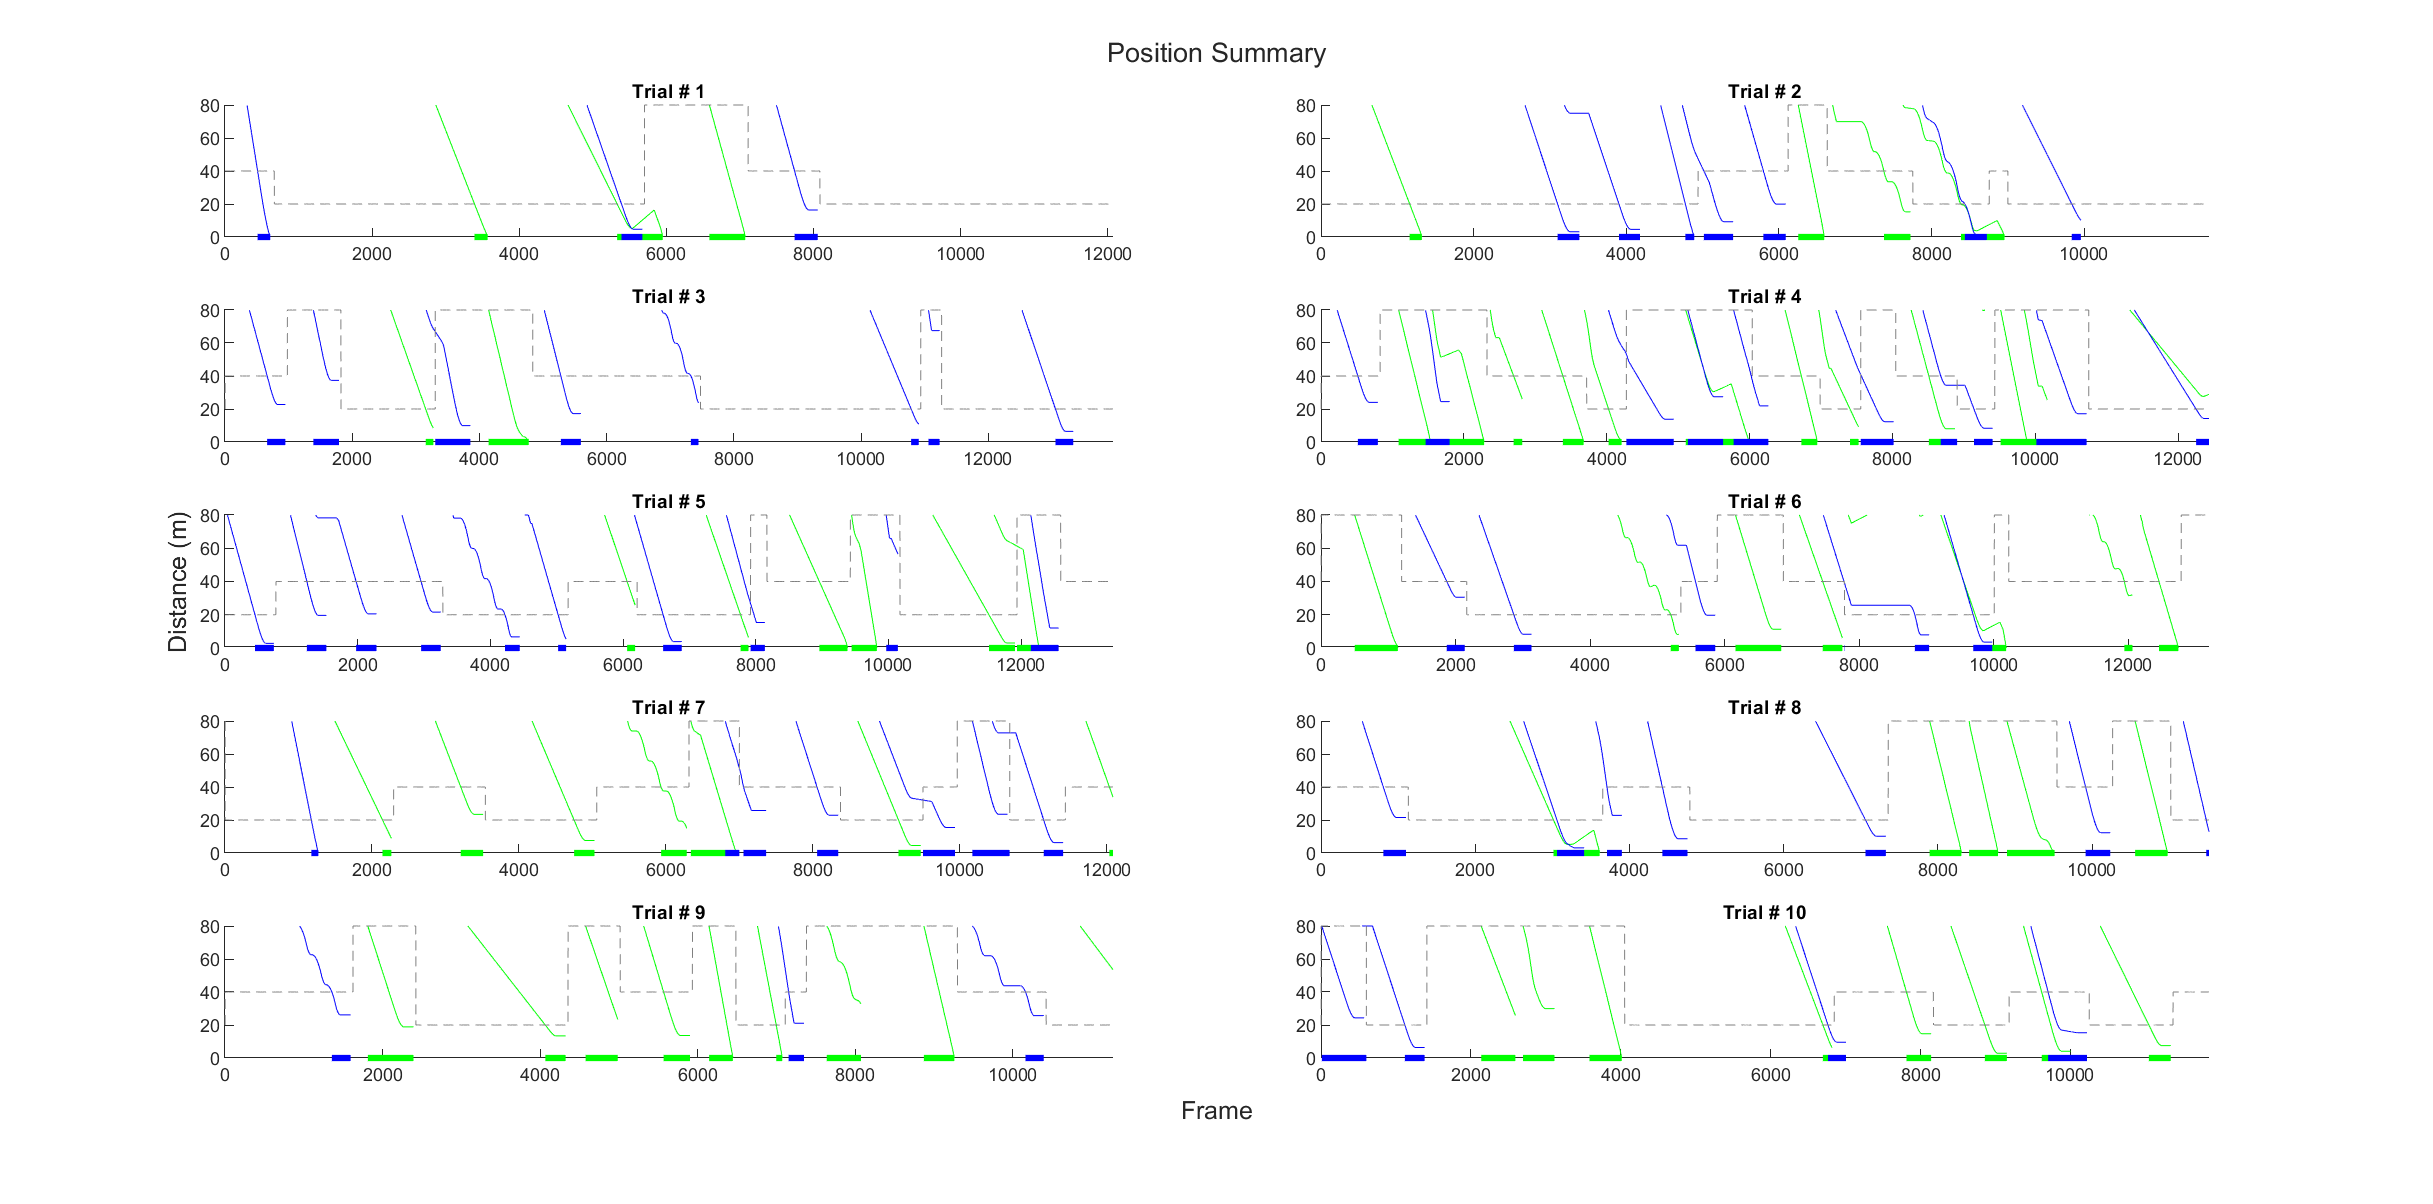
\includegraphics[width=\linewidth, height=\plotHeight\linewidth]{figures/subject_f_summary.eps}
    \caption{Summary Plot of Subject F's Trials}
    \label{fig:SumF}
\end{figure}

% \section{This is how you title a subsection}

\end{appendices}